\documentclass{article}

% 10-703 Style requirement.
% This will set margins, and make the look-and-feel of the document a research paper
\usepackage[final]{nips_2017}
%%Some semiuseful packages
\usepackage[utf8]{inputenc} % allow utf-8 input
\usepackage{amsmath}
\usepackage{amssymb}
\usepackage{fancyhdr}
\usepackage{graphicx}
\usepackage{tikz}
\usepackage{stmaryrd}
\usepackage{enumerate}
\usepackage{fancyvrb}
\usepackage{subcaption}

\usepackage[english]{babel}
\usepackage[backend=bibtex]{biblatex}
\addbibresource{FinalReport.bib}

\title{Creating Human-like Fighting Game AI through Planning}

\author{
  Roger Liu \\
  Carnegie Mellon University \\
  \texttt{rogerliu@andrew.cmu.edu} \\
}
%\date{Due: 28 January 2016}
\begin{document}
\maketitle

\begin{abstract}
Games are a major testing ground for Artificial Intelligence. Though AI has become proficient at playing games such as Space Invaders, it behaves in a way that is distinctly artificial, lacking the human-like qualities of a real player. This human element is important in competitive multiplayer games, as a large part of the enjoyment comes from outwitting other human strategies. To address this issue, we investigate a novel AI technique that leverages planning and human demonstrations to create an opponent that exhibits desirable qualities of human play. We introduce the idea of $\Delta$-actions, which the AI uses in order to figure out the causal relationship of actions and the game state. These $\Delta$-actions are learned from human demonstrations and are used to help the AI plan out a strategy for hitting the opponent. We implement a simple fighting game called \textit{FG} for the AI to compete in and provide it a human demonstration to learn from. Lastly, we evaluate the effectiveness of our AI by comparing its similarity score against other algorithms' and other demonstrations by the same human player.
\end{abstract}




\section{Introduction}
Fighting games are unique among competitive games in that they are real-time, 1-on-1 games where small mistakes lead to huge consequences. The best way to get better at these kinds of games is to practice against other humans, but that is not always an option. While online play exists, is not ideal because of network latency. In addition, the AI in these games are generally considered a poor substitute. They often exploit natural advantages such as perfect reaction time and perfect game state information, but even disregarding that they still only have fixed spectrum of behavior patterns which players can learn to exploit and consistently defeat. Worse still is that these behavior patterns might not even be representative of the human opponents that players encounter in competition.

That said, there are avenues to improve the AI in fighting games to make them useful for players. One approach is to make an optimal AI which is able to adapt its strategy based on its performance. This would provide players a challenge by removing the ability to exploit the AI, but it still doesn't necessarily capture the strategies and techniques used by other human players. Another approach is to make a \textit{human-like} AI, one that plays like another specific human opponent. This task seems feasible, as long-time fighting game players can identify the differences between the playstyles of different players, meaning that there is some quality that differentiates one behavior from another.

In this research, we investigate planning-based approaches to creating human-like AI. To do this, we first explore previous approaches taken to create human-like AI and discuss their merits and limitations. We also describe other attempts at creating AI for fighting games to contextualize our efforts compared to theirs. We then introduce the environment we created to test our approach and define concepts and terminology used by our algorithm. Lastly, we describe our algorithm, where we plan on the actions provided by human demonstrations to reach a desired outcome.









\section{Related Work}

\subsection{Racing and Imitation}
One of the few documented instances of Imitation AI came from the racing game \textit{Forza Motorsport}. In this game, players could train "drivatars" to race just like themselves. This was implemented by having the AI learn how the player behaves on different segments of track and try to replicate that behavior when it encounters those sections. However, this imposed a restriction on the types of tracks that could be present in the game, as they had to be formed from the basic segment building blocks.

Researchers then expanded on this approach through the use of genetic algorithms [DrivingPlayerModeler]. In these kinds of algorithms, candidate solutions are continually evolved toward better solutions. These candidates have a set of parameters which are altered between each iteration of the process, and are then evaluated according to a fitness function. For the particular case of creating robust human-imitating racers, a fitness function made up of 3 different components was used. 1 focused on matching the players progress on the track. Another focused on it matching the player's steering and a final one had it match the player's speed. The resulting AI did an alright job of mimicking some aspects of the repsective players, as the AI imitating a slow, careful driver behaved in a significantly different way from the faster, reckless driver. However, closer inspection of the driving AI showed that the resulting behavior was not conceivably human. Later attempts which had the fitness function that incoporated a focus on having the AI drive optimally also did not obtain convincing results, but it showed a clear trade-off between driving optimally and improving driver similarity. [MultiObjectiveMimic]

\subsection{Super Mario Bros.}
Researchers also developed several methods to mimic human behavior is in the space of 2D platformers, specifically a modified version of Super Mario Bros. [MarioImitation]. Novel methods tested in this space were Inverse Reinforcement Learning and Neuroevolution. 

The results of the Inverse Reinforcement Learning approach were discouraging, as the agent wasn't able to consistently handle situations that weren't often seen in the demonstration and was unable to match a human's ability to predict things not in the immediate detection area. In addition, the optimal policy obtained by IRL is deterministic, further reducing the human-like appearance of the AI.[MarioImitiation2]

Neuroevolution produced much better results. In this method, a neural network was first trained to play Super Mario Bros. The state of the game was encoded into various genre specific variables that denoted the state of Mario and the distance of Mario to various obstacles. This was handed as input to the neural network, which was then expected to output the buttons that should be pressed in that situation. The resulting weights were then evolved and evaluated using a fitness function. The fitness function in this case was the distance between the AI and player's traces through the level. A key improvement made to suit this genre was to reset the AI's position once the distance exceeded some threshold and apply a flat penalty. This is because an AI can easily get stuck in a 2D platformer, leading to a very bad final fitness score. The result was that the AI did the best job of mimicking human playstyles compared to many other algorithms. However, the agent achieved a lower score in the game compared to human players, showing that the agent had not really achieved a truly human-level of performance in the game.

\subsection{Fighting Games and Neural Nets}
Neuroevolutionary techniques have also been applied to fighting games. On a simple fighting game with 1 axis of movement, researchers found that evolutionary neural networks were able to quickly converge to an optimal playstyle [FightingAIComparison]. Additionally, Deep Reinforcement Learning has been able to create AI agents that can compete with top players in the popular commercial game Super Smash Bros. [SuperSmashBros]. However, optimal AI are not ideal substitutes for playing against human opponents. In the case of the Deep RL AI, it was specifically trained against only one kind of opponent, meaning that it was limited in the range of matchups it could perform well in. In addition, it exhibits obviously artificial traits such as impossible to perform back and forth movements.

\subsection{Ghost AI}
With regards to creating AI that was specifically human-like, the most notable attempt was something called Ghost AI, which was implemented on a version of the commercial game Street Fighter. This AI essentially initializes a table with the frequencies that the target player did a move and then used those moves at the same frequency[Ghost AI]. In the adaptive version, the AI would update the frequencies based on the reward gained from performing those moves [Ghost AI2]. 

To evaluate this AI, they recorded player sessions and sessions of the corresponding mimicked AI. The players were then asked to watch these recored sessions and perform inputs as if they were in the same situation. The recordings were then scored by the similarity of the recordings inputs to the "fake" test subject inputs. By this evaluation metric, this method showed promising results, as it was able match around 75\% of the real recordings accuracy. Players also expressed high qualitative satisfaction with their recordings, and the adaptive component allowed the AI to adjust itself to the strategies of the opponent. This approach has some notable pitfalls, as it does not account for specific player strategies that include varying timing. It also fails to account for contextual information, such as position on the screen, which factors into the decision making process for a real human player. 

\subsection{Data-driven Finite State Machines}
One final approach that to this problem was to create Data-Driven Finite State Machines. In this method, a multi-layered finite state machine is formed from the a log of a human demonstration. Specifically, the moves performed during the demonstration are annotated and used as designations for the AI states that it transitions between.

This approach has some clear limitations. For one, the annotation of moves is cumbersome and not well suited for a general purpose algorithm. Furthermore, the strategy that a player uses could be determined by an arbitrary number of in-game and out of game variables, which makes reducing player behavior to an FSM an daunting task. Lastly, this method was implemented on a 1D fighting game, which puts a huge limitation on the types of techniques that can be expressed by players.

\subsection{High Level Overview}
In this section we discussed several different existing methods for creating AI that mimic human-behavior. In domains where players progress on a path to an objective, such as racing games and 2D platformers, neuroevolution proves to be a strong strategy. However, there is a clear tradeoff between improving similarity and improving performance in these games, and even then these AI's have a hard time recovering from getting stuck. 

When looking specifically at fighting games, there is currently a lack of new developments. Though neural methods have proven effective at creating optimal agents in certain environments, they exhibit traits that prevent them from being suitable substitutes for human players. Other techniques such as Ghost AI have demonstrated an ability to express traits of human play, but lack the capability to account for the in-game situation in a human-like manner.


\section{Motivation for Planning-based Approach}
A commonality of all of the previous algorithms is that they all use some degree of learning to try to determine the best actions to take at any given situation. However, this approach has some issues. For one, learning requires a large amount of training in order to generalize across the large state space. This is problematic, as the player data gathered over multiple sessions is relatively small. Additionally, because the agent only learns the best actions to take at the current time step, it lacks the ability to plan for a sequence of actions that form a cohesive strategy. This part is important, as individual playstyles are categorized by the strategies that a player tends to use. Lastly, there is a natural trade off between optimality and employing a degree of randomness when these agents decide the next action to take. If an AI always does the same action in response to a situation, it loses the unpredictability of human play. However, if an AI does a random action that is unreasonable for the current situation, players will instantly recognize it as an AI. 

\begin{figure}[h]
	\centering
	\begin{subfigure}[h]{0.4\textwidth}
		\centering
		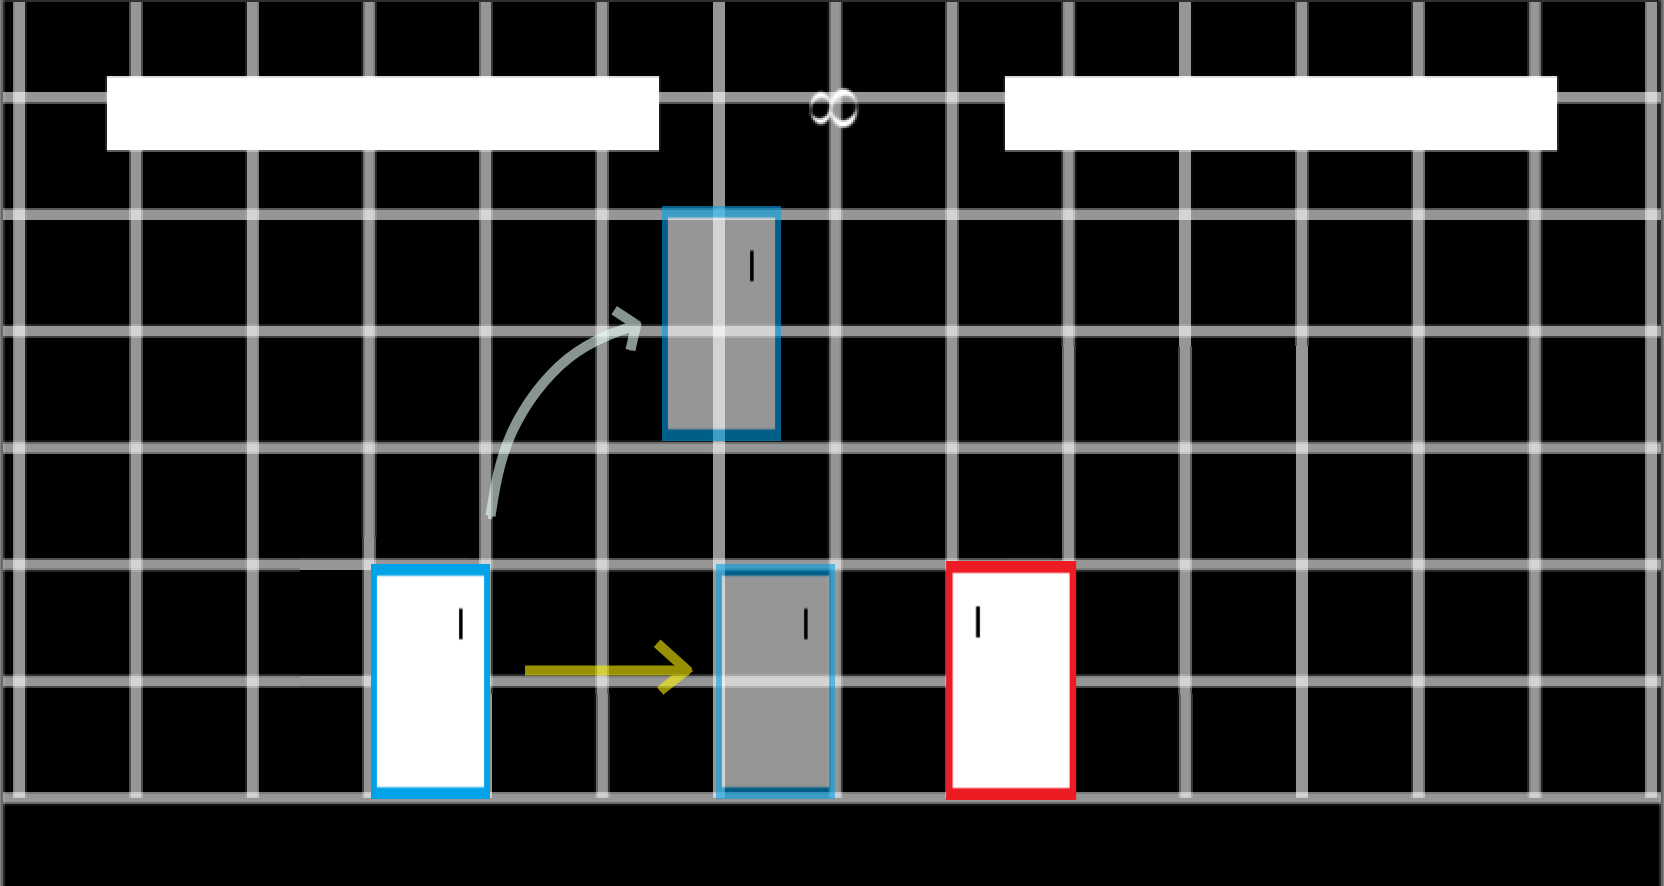
\includegraphics[width=\textwidth]{LearningExample1.png}
		\caption{Not varying actions}
		\label{Learning1}
	\end{subfigure}
	\begin{subfigure}[h]{0.4\textwidth}
		\centering
		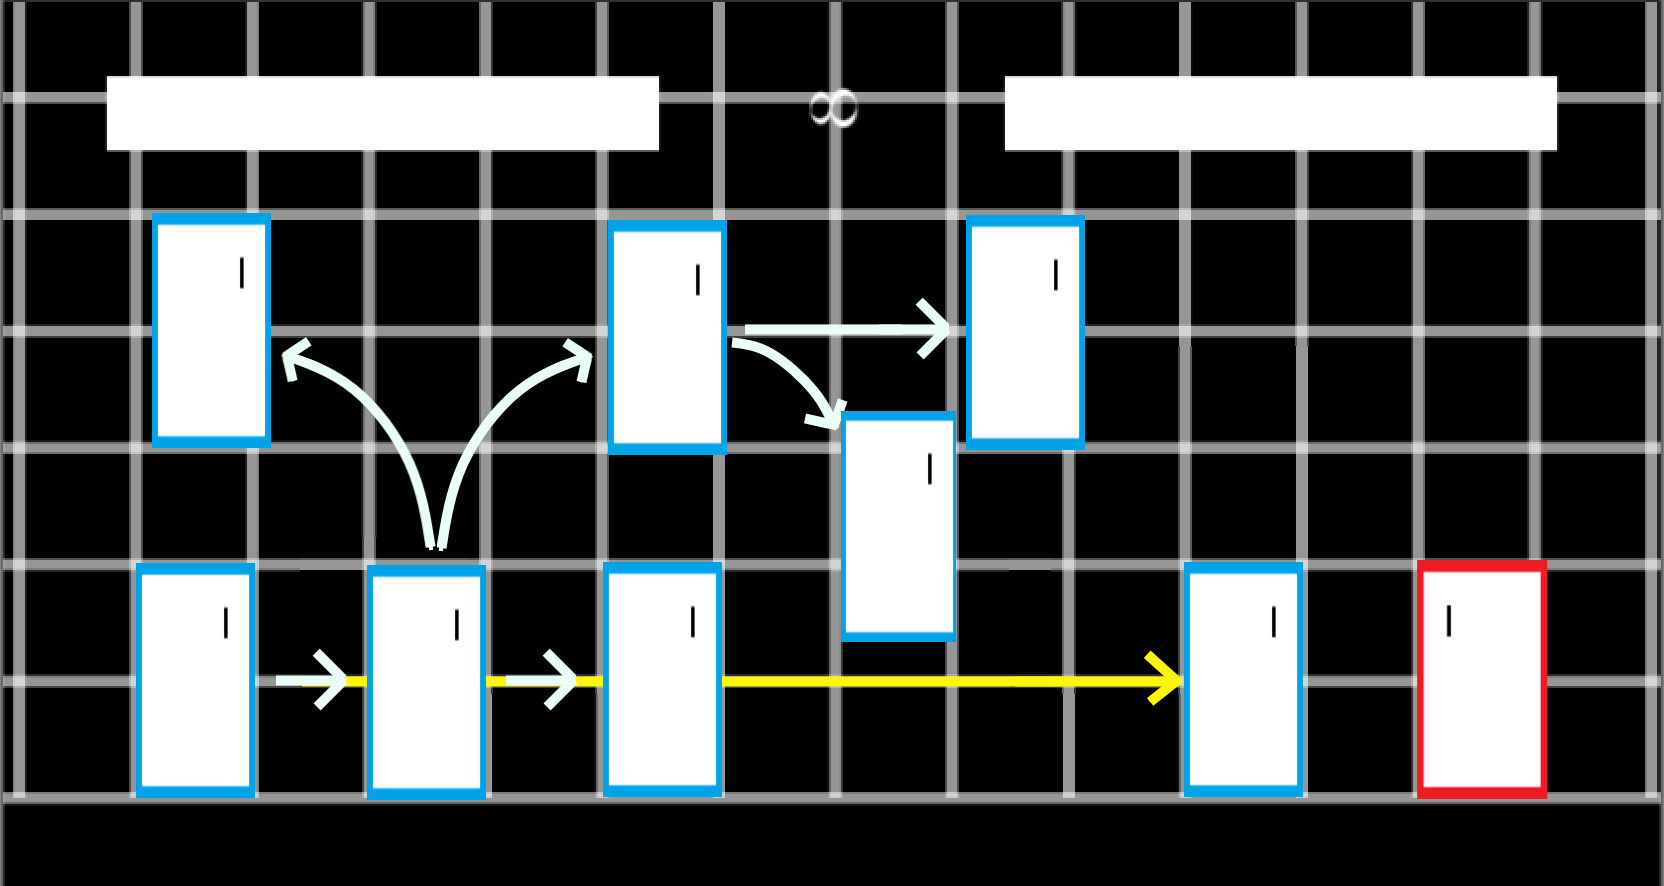
\includegraphics[width=\textwidth]{LearningExample2.png}
		\caption{Many points of failure}
		\label{Learning2}
	\end{subfigure}
\end{figure}

%This is because while learning techniques are very good at determining the right move to make given a situation, they don't do a great job at planning long-term strategies. 

%Even if the algorithm learns the distribution of the actions that the player tends to take, a chain of selections would still be unlikely to form something that resembles cohesive strategy. This is because the AI has to decide on an action to perform on every frame. This ultimately results in the jittery movements that characterizes these kinds of AI's in dynamic environments, as it's hard for it to decide to do a single action for a prolonged period of time.

\subsection{Why Use Search?}

Because human-play is heavily predicated on the usage of different kinds of strategies, an human-mimicking AI should dynamically create and execute strategies in the same way as the target player. Since strategies are essentially a sequence of actions that a player takes in order to arrive at a desired goal, the formulation of strategies can naturally be represented as a search problem over the state space. The target player's demonstrations can be used to guide to search, and custom heuristics can bias the search towards more closely mimicking the player. In addition, the demonstrations can be used to create a model of the game state's dynamics, which allows us to form cohesive plans even with relatively little training data.

%Though split second decision making is an important part of playing fighting games, human-play is also characterized by a tendency to rely on a set of strategies to defeat an opponent. To understand why search might be better able to capture these strategies, consider the following strategy

\begin{figure}[h]
	\centering
	\includegraphics[width=\textwidth]{Flowchart.png}
	\caption{Flowchart}
	\label{Player Strategy}
\end{figure}

In the demonstration, player 1 tends to try to stay within a certain range of the opponent and try to hit them with a low attack. If the opponent blocks the low attack, it sometimes then tries to jump in while the opponent can't move out of the way and hit them with a air attack. Essentially, player's 1 strategy is to try to reach a state where the opponent either gets hit by the low attack or is forced to try to block the air attack. There are 2 goals of this strategy, and reaching either of the goals requires performing a specific series of inputs.

In a learning context, the AI has to decide at each frame what action it must do. This means that as the AI is walking towards the opponent, it must decide at each frame that the correct action to do is walk left. However, this results in a series of issues on the implementation side. First of all, it requires that we must record the players action during every frame of a training episode, as otherwise unknown states would pop up all of the time as the player moves forwards. Further more, we quickly find that the AI performs poorly when starting in an unfamiliar position. This is because it is unlikely to find its way to a state that it has properly been trained on, and because it tries to pick an action to do at every frame, it is unlikely to reach a stable state and settle back into a correct strategy. Though function approximators can alleviate the tendency of the AI to take essentially random moves, it still is fairly ineffective at predicting the proper action in states that are unlike anything it's trained on. Though the initial demonstration can give the AI a pretty good idea of what to do when presented the exact same situation, it quickly falls apart the second we reach an unknown state. Compounded with the fact that we want to represent the game state with several categorical variables, this approach will likely fail to be robust enough to represent a human AI.

In the planning context, we can immediately remove a lot of the jittery randomness and uncertainty that plagues learning. By commitng to doing an action for a predetermined amount of time, we can guarantee consistent behavior like walking forward. In addition, since these actions are pulled directly from human demonstration and used in the plan based on their degree of usage, we are much more capable of performing the same kinds of actions as the player we are mimicking. Lastly, we are still able to quickly respond to movements by the opponent by simply replanning, essentially keeping the reactive benefits of the learning approach while not sacrificing on the consistency. 

\subsection{Unknown Situations in Search: Action Effects}

An issue that still is prevalent is that of robustness. When the AI encounters a state that it hasn't seen before, what should it do? We propose to solve this issue using a technique we dub \textbf{action effects}. The idea is that many actions have easily predictable actions. For example, moving left for a long time will always move the player a certain distance to the left. This formulation works for this domain because the results of actions in fighting games are completely predictable, as it's all codified inside the game engine. 

What does one do with these action effects? Well, we can use them to give the AI an idea of what to do in a state it hasn't seen before

\begin{figure}[t]
	\centering
	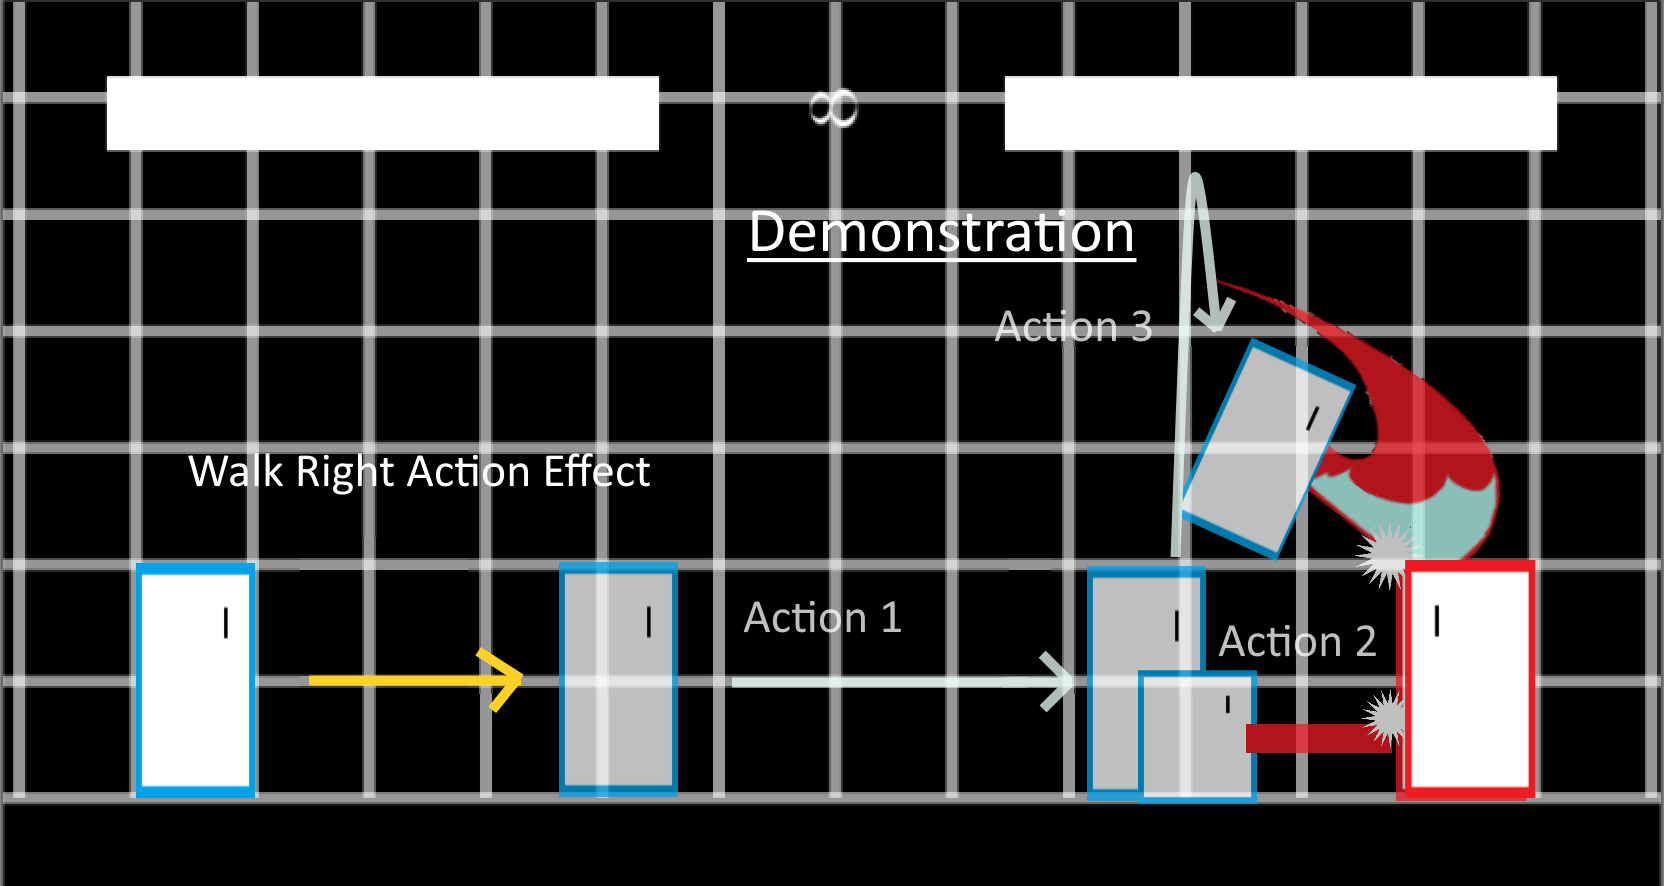
\includegraphics[width=\textwidth]{ActionEffect.png}
	\caption{Action Effects}
	\label{ActionEffects}
\end{figure}


For example, lets say that the player starts from far away from the demonstration etc etc.


\section{Algorithm Specifics: Fighting games as a search}

\subsection{System overview}
We created our own fighting game called \textit{FG} as as the testbed for this approach. This gave us complete control over the dynamics of the game. It also gave us access to internal game data which would have been considerably more difficult to access had we instead opted to modify an existing fighting game. 
	
The game is structured as a traditional fighting game. Players move back and forth on in a 2D space, trying to land blows on one another to reduce the opponents health to zero. There are a total of 21 \textbf{types} of actions that the player can, and each of these actions can be done for a duration which typically ranges from 1 to 40 frames (though for some actions like standing, the duration can be arbitrarily long). 
	
The game removes things like requiring complex inputs for special attacks, simplifying most fighting games to their core mechanics. The specific \textbf{types} of actions that players can take are described in Table \ref{actions}

\subsection{Algorithm Design and implementation}
In order to formulate the fighting game as a search problem, we need to discretize the state space as a graph. The nodes on this graph represent the game state at a specific point in time. This includes the positions of the players, their velocities, and various other metrics that capture their internal state. Full details can be found in Table \ref{gamestate}. The edges between nodes $a$ and $b$ represent transitioning from state $a$ to state $b$ via a \textbf{preformed action}. These are tuples which dictate an \textbf{type} of action that a player can perform and a \textbf{duration} that it is performed for. The set of actions that the AI can perform is restricted to the actions performed by the player in the training data. 

\subsection{Extracting performed actions}

During the training demonstrations, we record performed actions in the following cases

-When the player switches to a new action

-When the player is interrupted during the current action (ie. getting hit)

-When the game state changes during the current action

These actions are saved as a dictionary which maps the initial starting states of these actions to the final resulting state.

====Figures of examples of each case====

The last case is particularly important for the algorithm, as it breaks down the single player's action of walking forward into multiple smaller component actions that the AI can use.

\subsection{The successor function: utilizing Action Effects}

The last thing we need to do to fully define the search problem is to define the neighbors of any given state node $s$. If $s$ is a state we've seen in our demonstration, then we can easily use the transitions from $s$ found in the demonstration as the successors. 

==========Insert diagram of demonstration here============

However, the AI is likely to see states which were not seen during the demonstration. In these instances, we first determine the types of actions that are valid in the AI's current state. This rules out using impossible actions, such as walking forward while the AI is airborne. From the remaining action types, we find all performed actions in the demonstration with the matching action type and predict the result of doing that action in that state. These predictions are based on the action effects of those actions in the demonstration.

Specifically, the predictor is works as follows. To determine the effect of taking performed action $a$, we check our training data for all occurrences of that action. For each of those occurences, we extract the corresponding action effect. We then do a weighted average over all of the action effects to derive the final prediction. The weighting is set according to the similarities of the prior states for each action effect.

\subsection{Costs of Actions and Heuristics}
With the states, actions, and transitions defined, a cost function is required to be able to differentiate qualities of plans. The cost of all non-delta transitions is 1, as there is no qualitative way to evaluate one demonstrated action as being more "human-like" than another. For delta transitions, we employ a more sophisticated cost function.

TODO: Finalize the cost function and use it to enforce some kind of bounds.


\subsection{Goal states and Heuristics}
The final component we need to effectively perform search in this space is a goal state and heuristic function. 

Because our objective is to have the AI exhibit a certain kind of behavior, the goal state is only partially-specified. The function \textit{IsGoal()} determines whether a state is a goal state and is designed as follows.
 
Firstly, because this AI is intended to provide competitive players an more authentic representation of human play, the considered state must have the opponent in the \textit{FirstHit} status. Additionally, human players mix up their short-term strategies for getting hits so that they aren't predictable. To emulate this characteristic, we randomly select an instance in our demonstration where the opponent has the \textit{FirstHit} status and designate that as the \textbf{target}. We then require that the considered state has qualities similar to the target. This refers to the relative positions of the players and characteristics of each player's behavior states. 

For the heuristic, when evaluating state $s$, we took the Manhattan Distance of the relative positions of the 2 players and added that to the number of other parameters in $s$ which do not match the values in the target state $t$.

This \textbf{IsGoal()} function and the heuristic then gives us the following kind of behavior.

\begin{figure}[t]
	\centering
	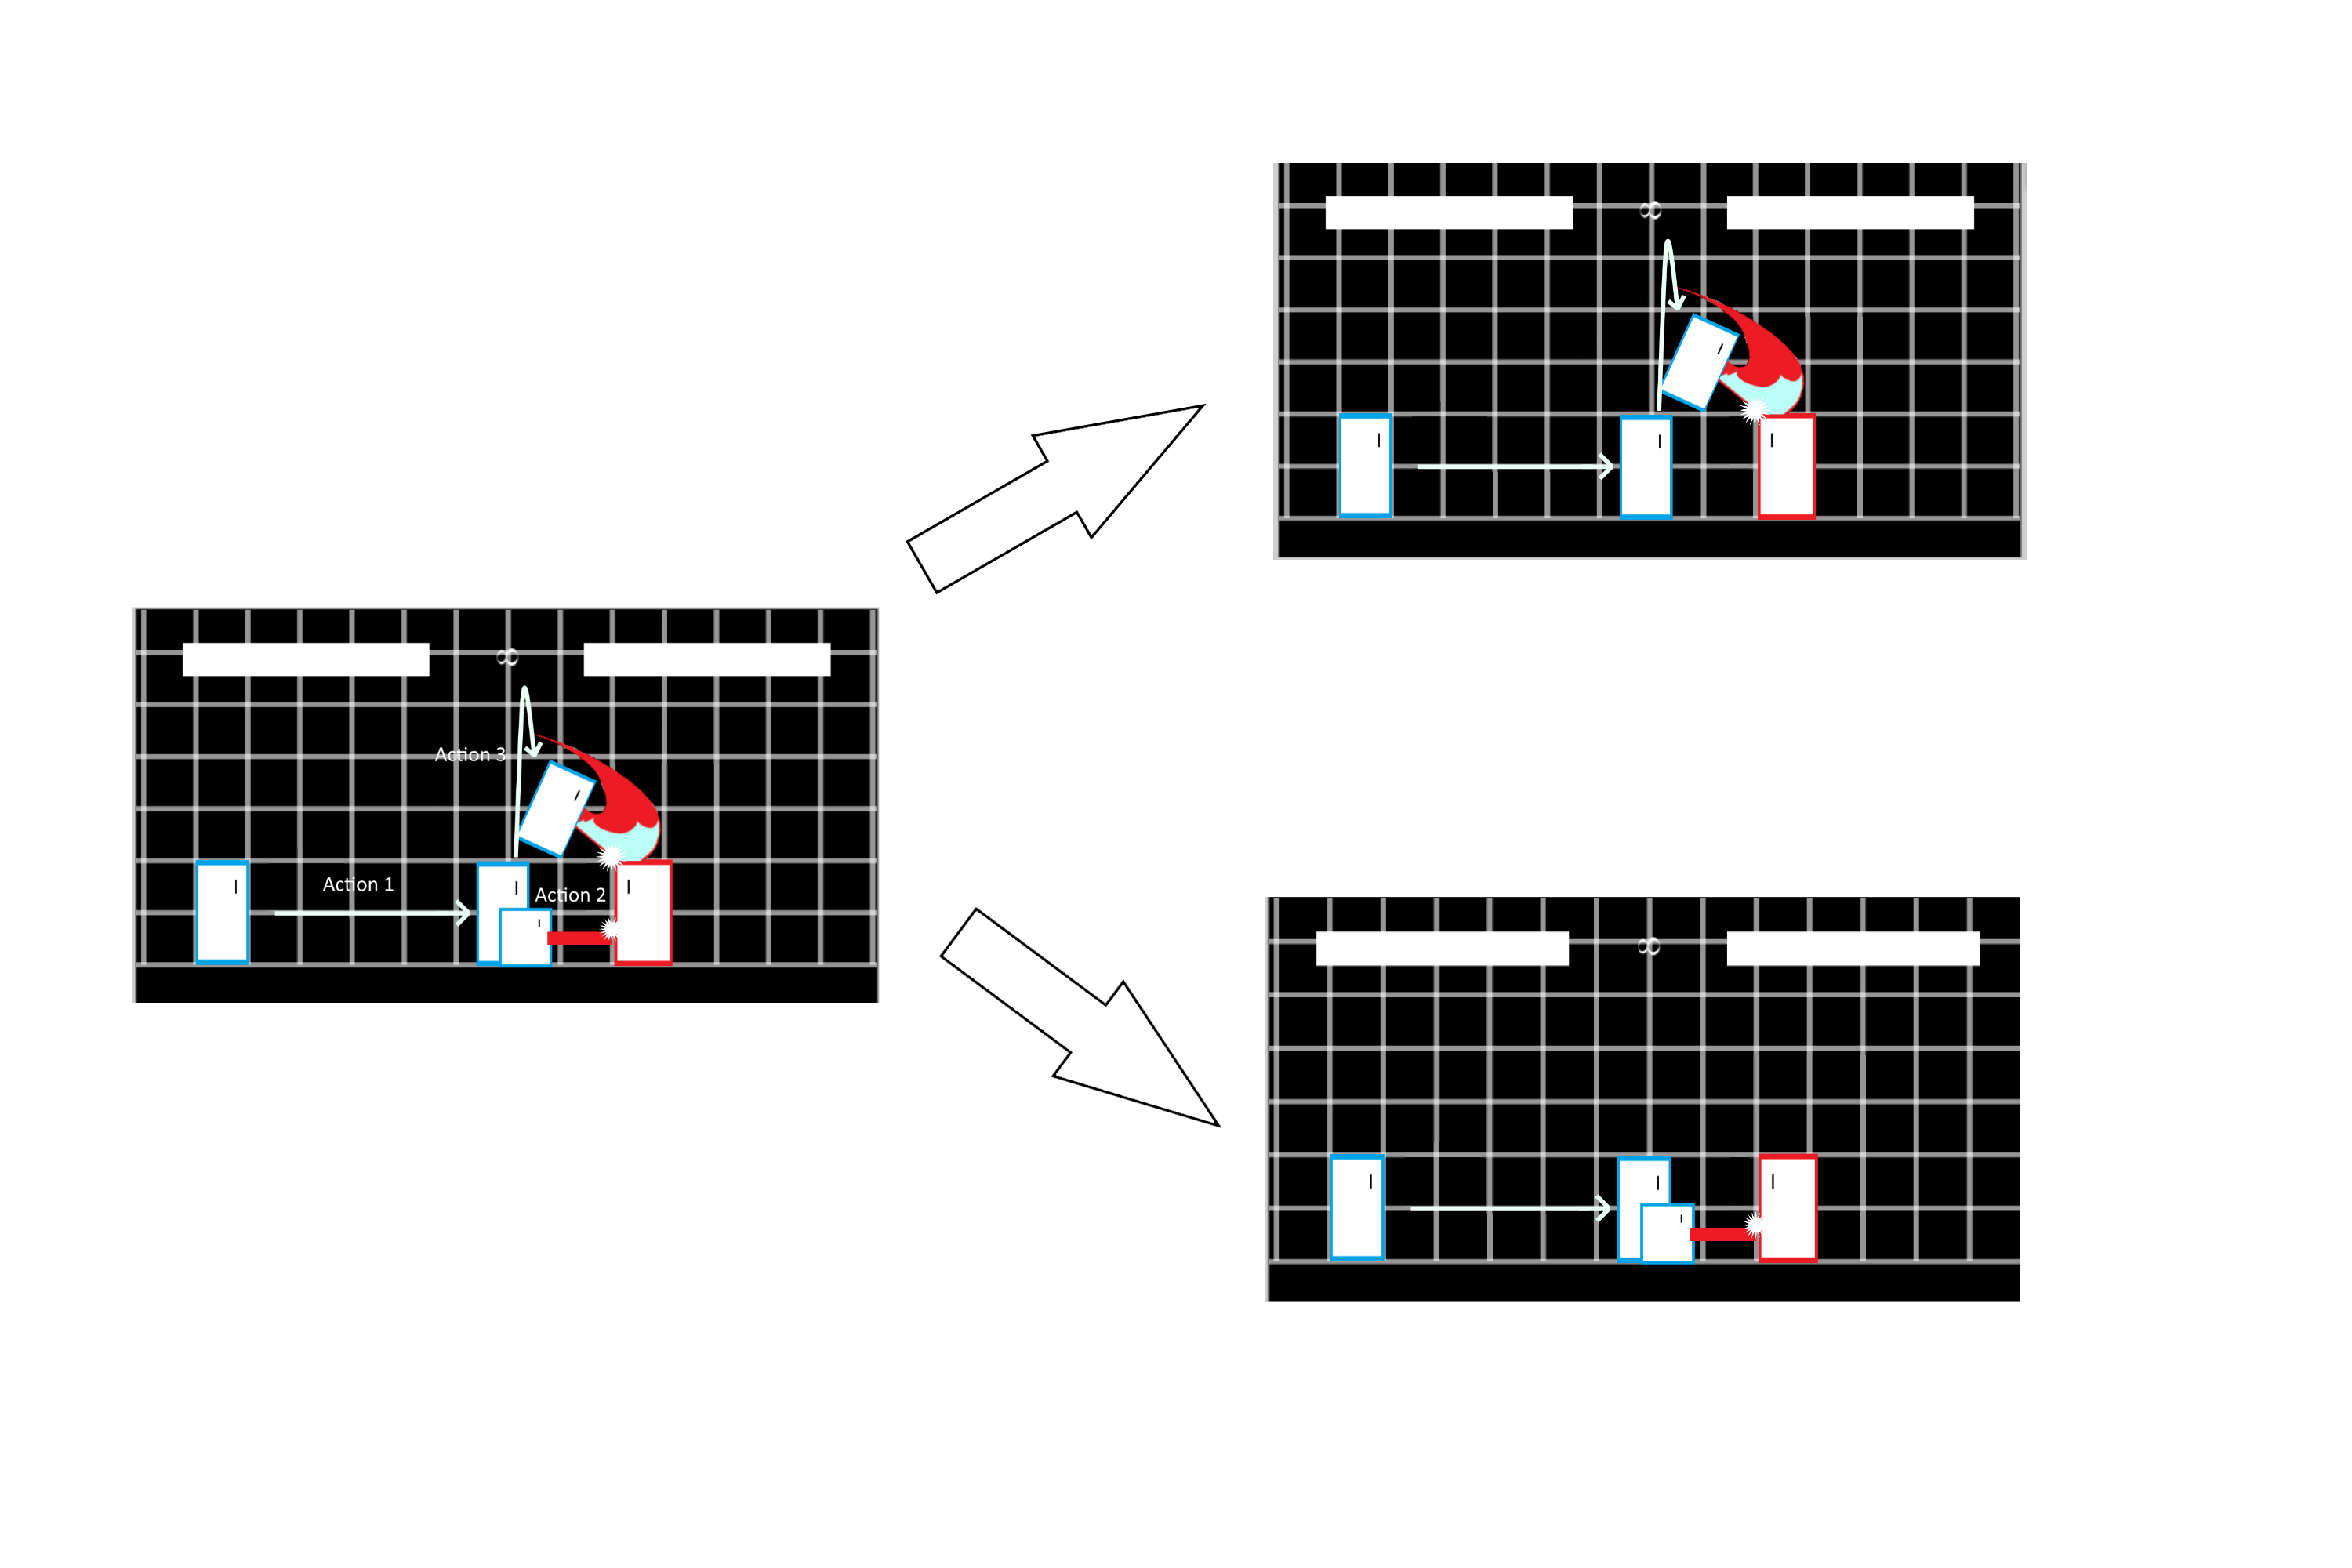
\includegraphics[width=\textwidth]{DecisionMaking.png}
	\caption{Action Effects}
	\label{ActionEffects}
\end{figure}

In the demonstration, we have one instance where the player hits the opponent with a low attack and another instance where the player hits the opponent with a jumping attack. One of the instances is randomly selected to be the target, and the AI then follows the appropriate plan to execute.


\subsection{Dealing with long search times: take the best available state}
Because of fast-paced nature of fighting games, players need to be able to reliably make split second decisions. This constraint then extends to our AI, as it can't afford to plan seconds at a time, as the game state might change drastically within that time period. In our implementation, the AI is required to come up with a plan within 50 milliseconds. If it cannot reach a goal state, it instead formulates a plan to get to the state with the highest projected value. The idea is that by reaching this intermediate state, it can then resume plannning from the position that is closer to the goal, giving the impression of one seemless plan, when it in fact generated that plan during execution.

\subsection{Dealing with a changing game state: replanning}
Because the opponent is allowed to move during plan execution, the plan we formulate is likely to encounter a state that we didn't expect. Because of the short time to plan we enforced, we can seemlessly replan whenever we hit an unexpected state and have the AI adjust accordingly. An example of this is when the opponent moves back while we're approaching them. Due to replanning, the AI will then know to continue to move towards the opponent, rather than stopping at it's original location and attacking like initially planned.

\subsection{Dealing with bad predictions, updating the predictor}
IN PROGRESS

\subsection{Interacting with the opponent, how to respond on defense}
IN PROGRESS
This might need its own subsection depending on how everything goes. Right now, results are promising for an offensive AI whose training data is a basic demonstration of high and low attacks, but we have yet to see if the AI can really respond to dealing with an actively moving opponent who will also attack it. Basically, will it learn to block? Do we have to do something to force it to learn to block?


\section{Results}

\section{Discussion}

\section{Additional Details}

\begin{table}[h]
	\centering
	\caption{AI Situation description}
	\begin{tabular}{| c | c |}
		\hline
		Field Name & Description \\
		\hline
		x Position        & Insert description here 	\\
		\hline
		y Position        & Insert description here 	\\
		\hline
		x Velocity        & Insert description here 	\\
		\hline
		y Velocity        & Insert description here 	\\
		\hline
		opponents x Position        & Insert description here 	\\
		\hline
		opponents y Position        & Insert description here 	\\
		\hline
		opponents x Velocity        & Insert description here 	\\
		\hline
		opponents y Velocity        & Insert description here 	\\
		\hline
		status        & Insert description here 	\\
		\hline
		opponents status        & Insert description here 	\\
		\hline
	\end{tabular}
	\label{gamestate}
\end{table}

\begin{table}[h]
	\centering
	\caption{Player Status descriptions}
	\begin{tabular}{| c | c |}
		\hline
		Status & Description \\
		\hline
		Stand & TEMP \\
		\hline
		Crouch & TEMP \\
		\hline
		Air & TEMP \\
		\hline
		Highblock & TEMP \\
		\hline
		Lowblock & TEMP \\
		\hline
		Hit & TEMP \\
		\hline
		KnockdownHit & TEMP \\
		\hline
		Tech & TEMP \\
		\hline
		Moving & TEMP \\
		\hline
		Dashing & TEMP \\
		\hline
		AirDashing & TEMP \\
		\hline
		StandAttack & TEMP When the opponent has the stand hitbox out\\
		\hline 
		LowAttack & TEMP When the opponent has the low hitbox out\\
		\hline 
		OverheadAttack & TEMP When the opponent has the overhead hitbox out\\
		\hline 
		AirAttack & TEMP  When the opponent has the AirAttack hitbox out\\
		\hline
		DP& TEMP When the opponent has the Dp hitbox out\\
		\hline 
		Recovery & The recovery period after an attack\\
		\hline
	\end{tabular}
\end{table}

\begin{table}[h]
	\centering
	\caption{Player Action descriptions}
	\begin{tabular}{| c | c |}
		\hline
		Action & Description \\
		\hline
		Stand & TEMP \\ 
		\hline
		Crouch & TEMP \\ 
		\hline
		WalkLeft & TEMP \\ 
		\hline
		WalkRight & TEMP \\
		\hline
		JumpNeutral & TEMP \\
		\hline
		JumpLeft & TEMP \\
		\hline
		JumpRight & TEMP \\
		\hline
		Attack & TEMP \\
		\hline
		Overhead & TEMP \\ 
		\hline
		LowAttack & TEMP \\ 
		\hline
		AirAttack & TEMP \\ 
		\hline
		StandBlock & TEMP \\ 
		\hline
		CrouchBlock & TEMP \\ 
		\hline
		DashLeft & TEMP \\ 
		\hline
		DashRight & TEMP \\ 
		\hline
		AirdashLeft & TEMP \\ 
		\hline
		AirdashRight & TEMP \\ 
		\hline
		DP & TEMP \\
		\hline
		TechNeutral & TEMP \\ 
		\hline
		TechLeft & TEMP \\ 
		\hline
		TechRight & TEMP \\
		\hline
	\end{tabular}
	\label{actions}
\end{table}

\printbibliography

\end{document}
